\section{Laplace-Transformation}{135}

Die Laplace-Transformation kann als analytische Fortsetzung der Fourier-Transformation aufgefasst werden. \\
Die Frequenz ist nun komplex $\cbl{(s = \sigma + \jimg \omega)}$ anstelle $\jimg \omega$. Dank dem Dämpfungsfaktor $\sigma$ kann die
Konvergenz von Signalen erzwungen werden.


\subsection{Berechnung der Laplace-Transformation}{135}
\label{Berechnung der Laplace-Transformation}

Komplexe Frequenz: $s = \sigma + \jimg \omega $

$$ \boxed{\text{Laplacetransformation: } F(s) = \int\limits_{0_-}^{\infty} f(t) \, e^{-st} \, \diff t  } $$
$$ \boxed{ \text{Rücktransformation: } f(t) = \frac{1}{2 \pi \jimg} \int\limits_{c - \jimg \infty}^{c+ \jimg \infty} F(s) \, e^{st} \, \diff s  } $$

\textrightarrow\ Für die Rücktransformation werden meistens Tabellen verwendet!


\subsection{Eigenschaften der Laplace-Transformation}{136-138}

\subsubsection{Rechenregeln}

{\renewcommand{\arraystretch}{2}
\begin{tabularx}{\columnwidth}{@{}>{\raggedright\arraybackslash}X >{$\displaystyle}c<{$} c >{$\displaystyle}c<{$}@{}}
	\toprule
	\textbf{Eigenschaft} & f(t) & & F(s) \\
	\midrule
	Linearität ($\alpha, \beta \in \mathbb{C}$) 	& \alpha f(t) + \beta g(t) 	& $\laplace$ & \alpha F(s) + \beta G(s) \\
	Ähnlichkeit ($0 < \alpha \in \mathbb{R}$) 	& f(\alpha t) 				& $\laplace$ & \frac{1}{|\alpha|} F\Big(\frac{s}{\alpha}\Big) \\
	Verschiebung Zeit$^{(1)}$ 		& f(t \pm t_0) 				& $\laplace$ & F(s) \, e^{\pm t_0 s} \\
	Verschiebung Frequenz (Dämpfung) & f(t) \, e^{\mp \alpha t} 	& $\laplace$ & F(s \pm \alpha) \\
	Ableitung Zeit 					& \frac{df(t)}{dt} 			& $\laplace$ & s F(s) - f(0_-) \\[6pt]
									& \frac{d^2 f(t)}{dt^2} 	& $\laplace$ & s^2 F(s) - s f(0_-) - f'(0_-) \\[6pt]
									& \frac{d^n f(t)}{dt^n} 	& $\laplace$ & s^n F(s) - \sum_{k=1}^{n} s^{n-k} f^{(k-1)}(0_-) \\[6pt]
	Multiplikation mit $t$ 			& t \, f(t) 				& $\laplace$ & -\frac{dF(s)}{ds} \\[6pt]
	Ableitung Frequenz ($n \in \mathbb{N}_0$) & (-t)^n f(t) 	& $\laplace$ & \frac{d^n F(s)}{ds^n} \\
	Integration Zeit 				& \int_0^t f(\tau) \, d\tau 	& $\laplace$ & \frac{F(s)}{s} \\
	Faltung Zeit$^{(2)}$ 			& f(t) * g(t) 				& $\laplace$ & F(s) \cdot G(s) \\
	Faltung Frequenz 				& f(t) \cdot g(t) 			& $\laplace$ & \frac{1}{2\pi\jimg} \int_{c-\jimg\infty}^{c+\jimg\infty} F(\xi) \, G(s-\xi) \, d\xi \\
	\bottomrule
\end{tabularx}}

\vspace{0.1cm}

{\small
$^{(1)}$ Minus: wenn $t_0 > 0$ \quad Plus: wenn $f(t) = 0$ für $t < t_0$ \\
$^{(2)}$ $f(t) * g(t) = \int_{-\infty}^{\infty} f(\tau) \, g(t-\tau) \, d\tau = \int_{0}^{t} f(\tau) \, g(t-\tau) \, d\tau$}

\subsubsection{Grenzwertsätze}

{\renewcommand{\arraystretch}{1.8}
\begin{tabularx}{\columnwidth}{@{}l >{$\displaystyle}l<{$} >{\raggedright\arraybackslash}X@{}}
	\toprule
	\textbf{Anfangswert} 	& \lim_{t \to 0} f(t) = \lim_{s \to \infty} s F(s) 	& wenn $\lim_{t \to 0} f(t)$ existiert \\
	\textbf{Endwert} 		& \lim_{t \to \infty} f(t) = \lim_{s \to 0} s F(s) 	& wenn $\lim_{t \to \infty} f(t)$ existiert (Pole von $sF(s)$ in der linken Halbebene) \\
	\bottomrule
\end{tabularx}}


\subsubsection{Weitere Zusammenhänge und Tabellen}

\textrightarrow\ Siehe Skript Anhang 3.B


\subsection{Rücktransformation in den Zeitbereich }{139-141}

\textbf{\textrightarrow\ Meistens werden Tabellen verwendet!}


\subsubsection{Rücktransformation mittels Umkehrintegral}

\textrightarrow\ Siehe Abschnitt \ref{Berechnung der Laplace-Transformation}


\subsubsection{Rücktransformation gebrochen-rationaler Funktionen (PBZ)}

\myul{\textbf{Vorgehen Partialbruchzerlegung}}

\vspace{0.1cm}

\begin{enumerate}
  \item Nennerpolynom faktorisieren
  \item Bruch als Summe aus Faktoren schreiben
  \item Gleichsetzen mit ursprünglichem Term
  \item Koeffizientenvergleich (Zähler finden)
  \item Rücktransformation der einzelnen Summanden mit Tabellen
\end{enumerate}


\subsubsection{Rücktransformation mittels Residuensatz}

\textbf{ \textrightarrow\ Empfohlen für PBZ mit mehreren Polen}

$$ \boxed{ A_{ij} = \frac{1}{(n_i - j)!} \frac{\partial^{n_i - j}}{\partial s^{n_i-j}} \big[ (s-p_i)^{n_i} F(s) \big] \Bigg|_{s = p_i} } $$


\example{Residuensatz}

$$\text{Gegeben:} \quad  F(s) = Y(s) = \sum\limits_{i=1}^k  \sum\limits_{j=1}^{n_k} \frac{A_{ij}}{(s-p_i)^j} = \frac{6}{(s+4) \cdot (s+3)^2} $$
$$ \text{Ansatz PBZ:} \quad \frac{A_{11}}{s+4} + \frac{A_{21}}{s+3} + \frac{A_{22}}{(s+3)^2} $$

\begin{align*}
    A_{11}  &= \frac{1}{0!} \frac{\partial^0}{\partial s^0} (s+4) \cdot \frac{6}{(s+4) \cdot (s+3)^2} \Big|_{s = -4} = \frac{6}{(s+3)^2} \Big|_{s = -4} = 6 \\
    A_{21}  &= \frac{1}{1!} \frac{\partial}{\partial s} (s+3)^2 \cdot \frac{6}{(s+4) \cdot (s+3)^2} \Big|_{s = -3} =  \frac{\partial}{\partial s} \frac{6}{s+4} \Big|_{s = -3} = \frac{-6}{(s+4)^2} \Big|_{s = -3} = -6 \\
    A_{22}  &= \frac{1}{0!} \frac{\partial^0}{\partial s^0} (s+3)^2 \cdot \frac{6}{(s+4) \cdot (s+3)^2} \Big|_{s = -3} = 6
\end{align*}


% Von Zusammenfassung Integraltransformationen:
\subsection{Lineare DGL mittels Laplacetransformation lösen}
		
\subsubsection{Vorgehen: Lösen einer DGL mit Laplace}
		
\begin{enumerate}
    \item DGL inkl. Störfunktion $f(t)$ in Bildbereich transformieren \\
        \textrightarrow\ Anfangswerte für $f^{(n)}(0_-)$ einsetzen!
    \item Gleichung nach Laplace-Transofrmierter der gesuchten Funktion umformen
    \item Rücktransformation in den Zeitbereich
\end{enumerate}

		
\example{Lösung einer DGL mit Laplace}

\begin{minipage}[c]{0.6\columnwidth}
    \begin{tabular}{ll}
        DGL:            & $\ddot{y}(t) + 2 \, \dot{y}(t) + 5 \, y(t) = f(t)$ \\
        Anfangswerte:   & $y(0) = 0$; \quad $\dot{y}(0) = 0$
    \end{tabular}
\end{minipage}
\hfill
\begin{minipage}[c]{0.35\columnwidth}
    \textrightarrow\ Finde $y(t)$
\end{minipage}

\vspace{0.2cm}

\begin{enumerate}
    \setlength\itemsep{3pt}
    \item $\laplace \; s^2 \cdot Y(s) - s \cdot 0 - 0 + 2( s \cdot Y(s) - 0) + 5 \cdot Y(s) = 1(s)$ \\
        $s^2 \cdot Y(s)+ 2 \cdot s \cdot Y(s) + 5 \cdot Y(s) = 1(s)$
    \item $Y(s) = \frac{1}{s^2 + 2s +5}$
    \item Rücktransformation mit Tabellen
\end{enumerate}


% Aus Integraltransformationen
\subsection{Konvergenzhalbebene}
\label{Konvergenzhalbebene}

Es gibt jeweils mehrere (komplexe) Zahlen $s$, \textbf{für welche das Laplace-Integral konvergiert.} 
Die Konvergenzhalbebene beinhaltet alle diese Zahlen $s$

\vspace{0.2cm}

\begin{minipage}[c]{0.48\columnwidth}
    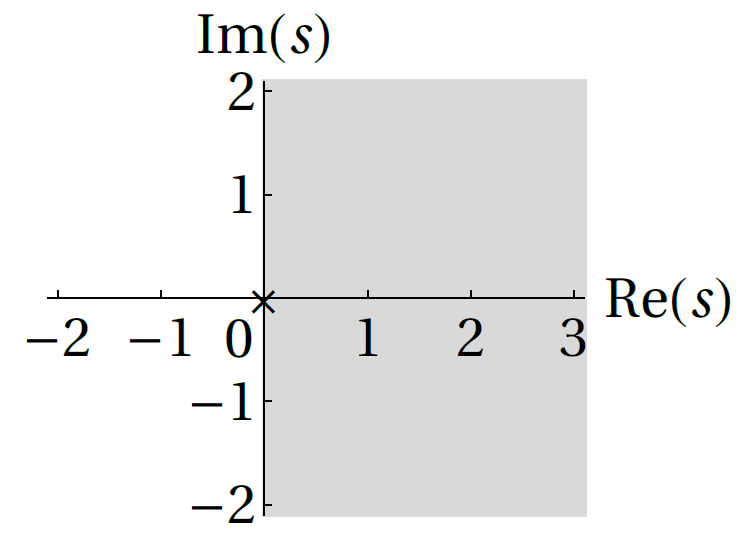
\includegraphics[width=\columnwidth]{images/konvergenzhalbebene.png} 
\end{minipage}
\hfill
\begin{minipage}[c]{0.48\columnwidth}
    Die Halbebene wird durch die \textbf{am weitesten rechts liegende Polstelle} von $F(s)$ begrenzt (Kreuzchen)
    \vspace{0.2cm}
    Falls $F(s)$ keine Polstelle hat, ist die Konvergenzhalbebene gleich $\mathbb{C}$
\end{minipage}


\subsection{Zusammenhang LT und FT}{145}

Bei kausalen, stabilen und fourier-transformierbaren Signalen $f(t)$ kann man durch das Ersetzen von $s = \sigma + \jimg \omega$ 
durch $\jimg \omega$ (und umgekehrt) zwischen der einseitigen Laplace-Transformation und der Fourier-Transformation wechseln.

\vspace{0.2cm}

Kennt man die einseitige Laplace-Transformation $F(s)$ des kausalen Signals $f(t)$, so kann man folgende Aussagen machen:

\vspace{0.1cm}

\begin{itemize}
    \setlength\itemsep{3pt}
    \item Liegt die $\jimg \omega$-Achse im Konvergenzbereich von $F(s)$, so kann $s$ 
        durch $\jimg \omega$ ausgetauscht werden, um $F(\jimg \omega)$ zu erhalten. 
    \item Liegt die $\jimg \omega$-Achse ausserhalb des Konvergenzbereichs von 
        $F(s)$, so konvergiert die Fourier-Transformation $F(\jimg \omega)$ nicht.
    \item Liegt die $\jimg \omega$-Achse auf dem Rand des Konvergenzbereichs von
        $F(s)$, so \textbf{können} die Fourier-Transformation $F(\jimg \omega)$ und die
        einseitige Laplace-Transformation $F(s)$ übereinstimmen, \textbf{müssen aber nicht}.
\end{itemize}
